\chapter{Autoencoders}
Gli autoencoder (AE) sono strumenti di apprendimento non supervisionato \textbf{utilizzati per migliorare le 
reti supervisionate} (ad esempio, utilizzando livelli di rappresentazione AE appresi per inizializzare la rete
supervisionata) e per \textbf{risolvere molti compiti interessanti}:
\begin{itemize}
  \item image colorization;
  \item increase resolution;
  \item image inpainting;
  \item machine translation.
\end{itemize}



Storicamente, sono state utilizzate, per esempio, per \textbf{ricolorare immagini}. L'input è la grayscale, 
e l'output è l'immagine ricolorata.
\begin{figure}[!h]
  \centering
  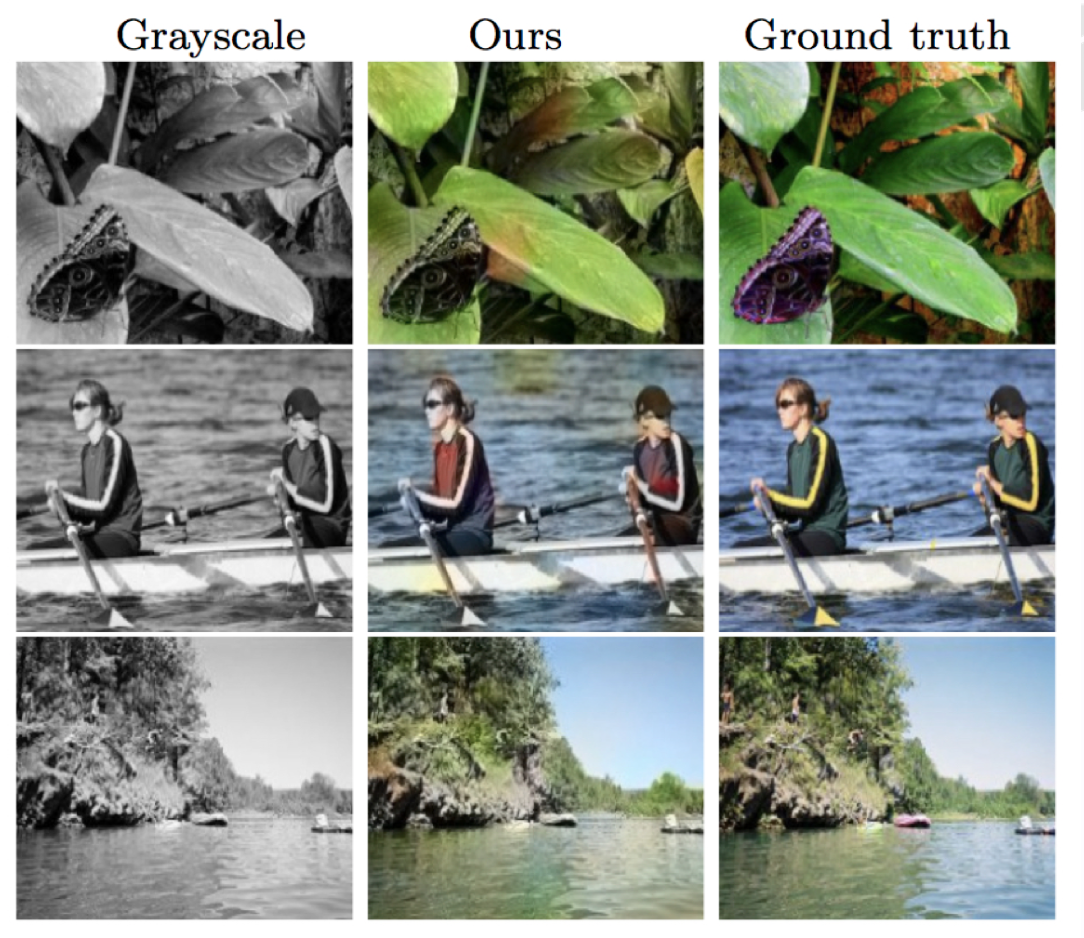
\includegraphics[scale=.3]{images/autoencoders/colorization.png}
\end{figure}

Un altro esempio di applicazione è dato dalla \textbf{increase resolution}, nel seguito applicata ad immagini.
\begin{figure}[!h]
  \centering
  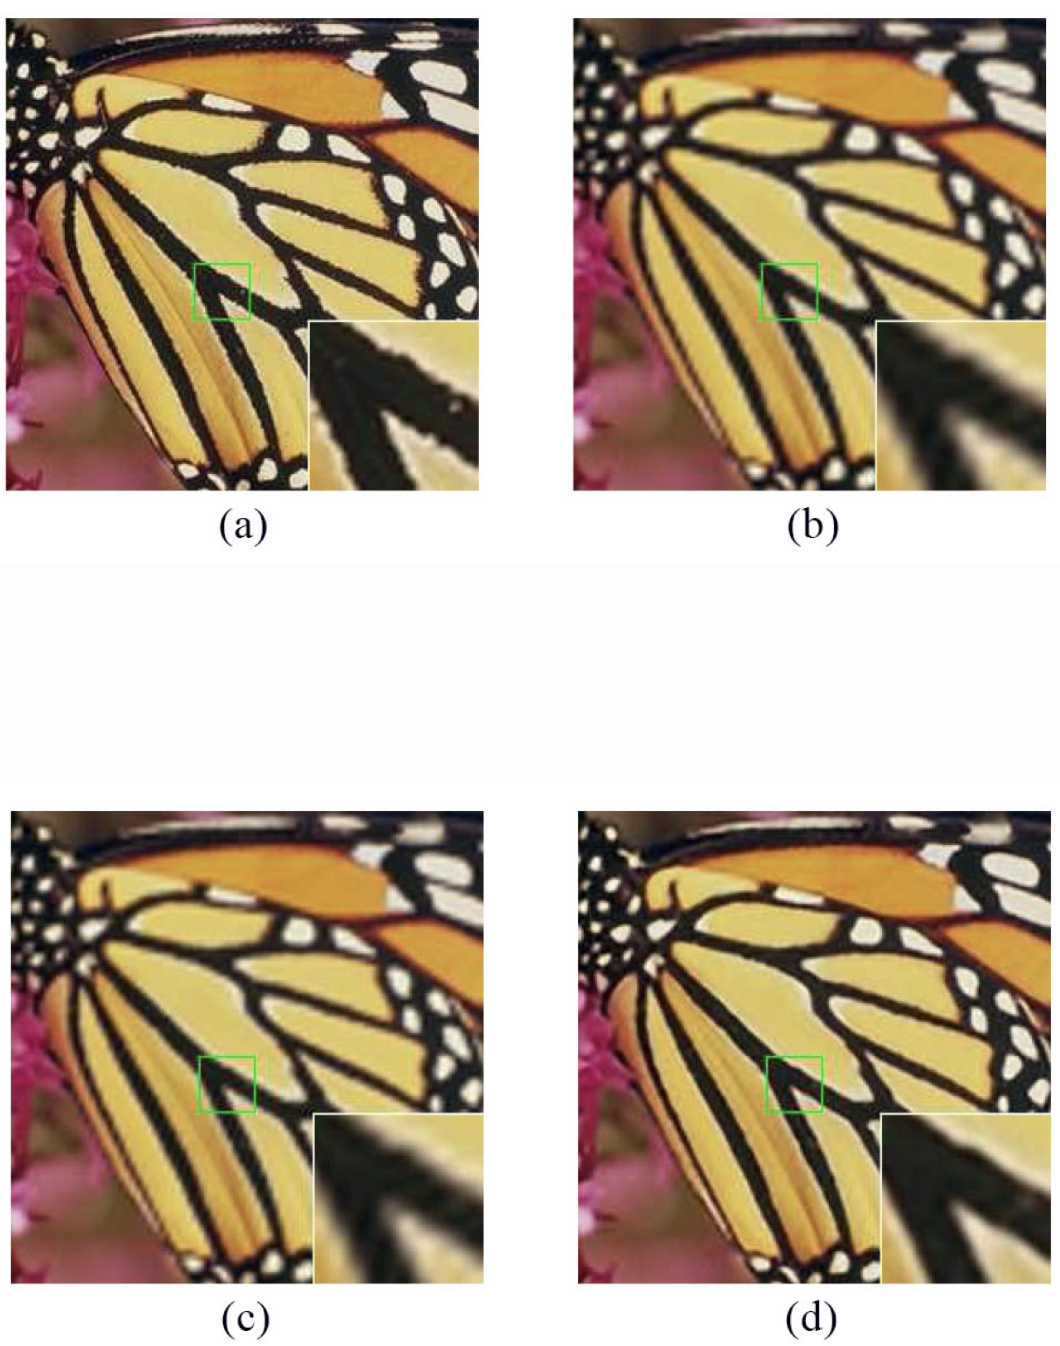
\includegraphics[scale=.27]{images/autoencoders/increase.png}
\end{figure}
\newpage

Oppure, ancora, \textbf{image inpainting}: l'input è un'immagine con background noise e l'obbiettivo è 
rimuoverlo.
\begin{figure}[!h]
  \centering
  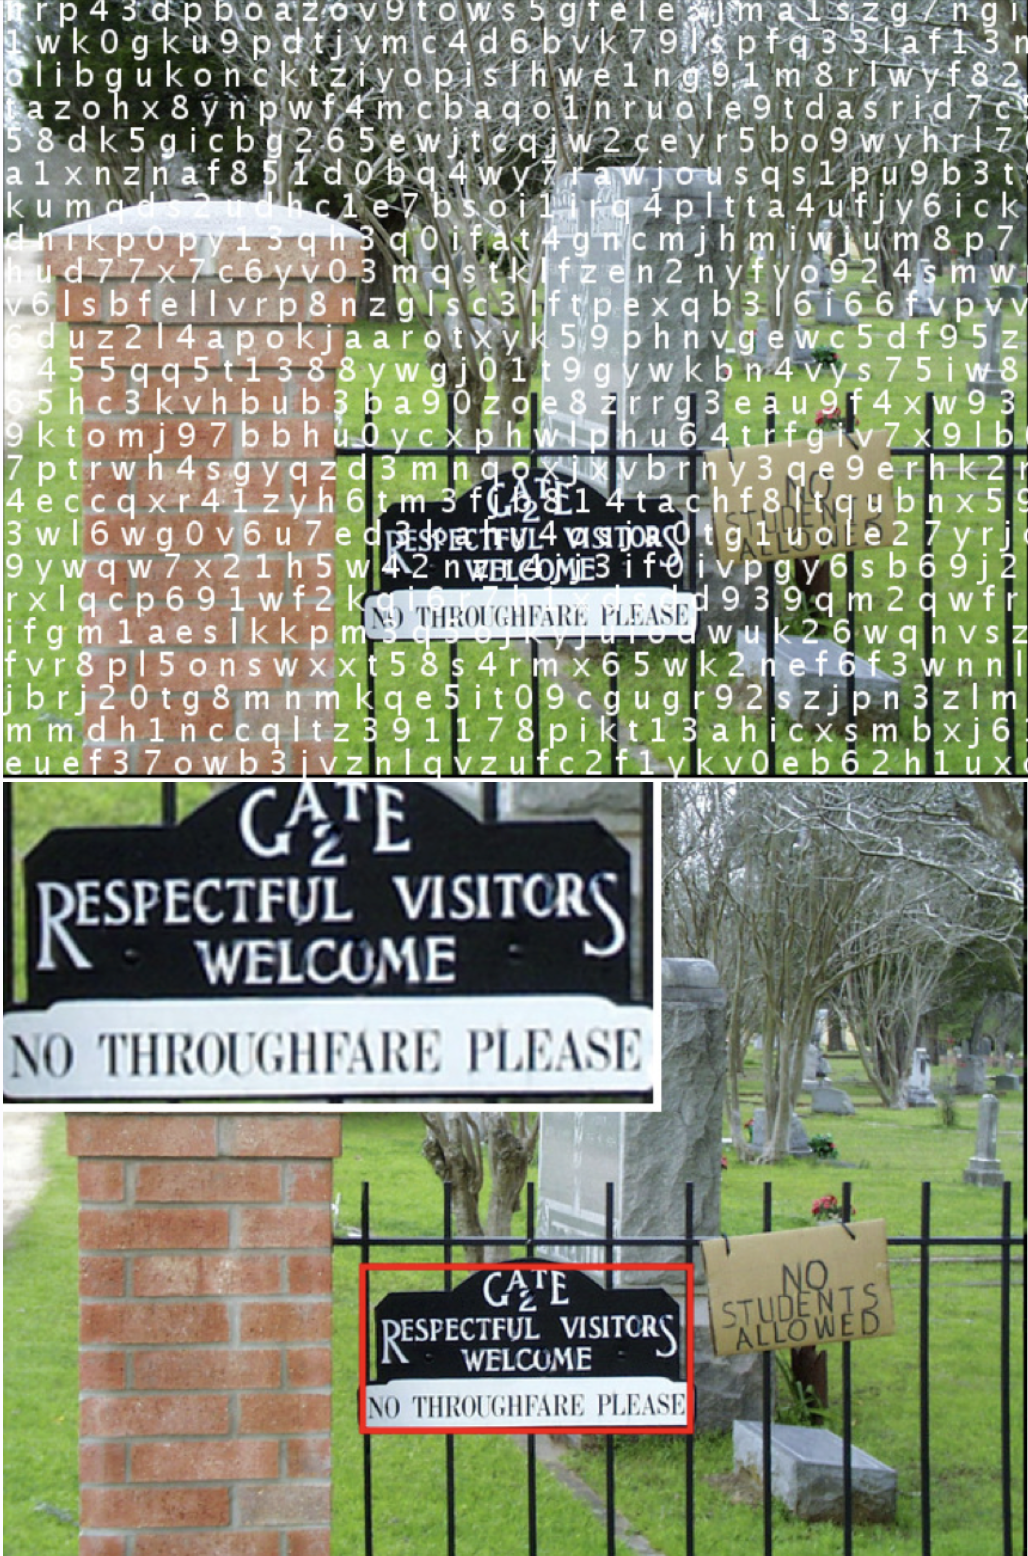
\includegraphics[scale=.27]{images/autoencoders/inpainintg.png}
\end{figure}

\section{Definizione}
Un autoencoder è una rete naturale addestrata a tentare di copiare il suo input nel suo output tramite una 
rappresentazione $h$ costruita dai suoi hidden layers. Se chiamiamo $h$ la \textbf{rappresentazione} e $x$ 
l'input, le componenti principali di un autoencoder sono:
\begin{itemize}
  \item \textbf{encoder} $h=f(x)$;
  \item \textbf{decoder} $r=g(x)$.
\end{itemize}
L'obiettivo dell'encoder è di costruire una nuova rappresentazione dell'input $x$, quello del decoder è invece
riprodurre l'input $x$. Può sembrare un processo stupido, miriamo a riprodurre l'input, ma ciò che è
importante è la rappresentazione. Nella nostra trattazione chiamiamo $f$ la parte dell'encoder, $g$ la parte
del decoder, $h$ la rappresentazione di $x$ e $\hat{x}$ la rappresentazione ricostruita di $x$.
Non è previsto che un autoencoder copi fedelmente ogni input nel suo output. Sono invece costretti a dare 
la priorità a quali aspetti dell'input dovrebbero essere preservati.
\newline
\newline
Tradizionalmente gli autoencoder sono stati utilizzati per la \textbf{riduzione della dimensionalità} o 
\textbf{l'apprendimento delle funzionalità}. Per quanto riguarda la dimensionality reduction, ad esempio 
si parte con un encoder che riceve una $x$ di 1000 feature e si costruisce una rappresentazione che ne ha 
100. Il punto è che l'autoencoder è pensato per essere in grado di riprodurre l'input, quindi la nuova 
rappresentazione, molto più piccola dell'originale, contiene comunque tutte le informazioni dell'originale,
perchè è stata costruita a partire dalle informazioni utili di essa.
\newline
Oggi sono la prima linea della ricerca sui \textbf{modelli generativi} grazie alle connessioni stabilite 
con i \textbf{latent variable models}.
\newline
\textbf{Nota:} un \textbf{latent variable models} è un modello che ha sia variabili osservate $x$ che 
variabili latenti $h$ e il cui obiettivo è apprendere la distribuzione $p(x, h)$. Abbiamo introdotto 
brevemente queste idee alla fine delle lezioni sull'apprendimento della rappresentazione.
\newpage

\section{Undercomplete Autoencoders}
Copiare Semplicemente l'input nell'output corrisponde alla costruzione della funzione identità, cosa che 
evidenetemente non è utile. Quindi la speranza è che durante il training si riesca ad imparare una qualche 
proprietà della hidden representation $h$ che sia utile.
\newline
Uno dei modi per ottenere una $h$ interessante è avere una $h$ con dimensioni più piccole di $x$. 

\paragraph{Definizione.} Un autoencoder la cui dimensione della codifica è inferiore alla dimensione dell'input
è chiamato \textbf{Undercomplete Autoencoders}.
\begin{figure}[!h]
  \centering
  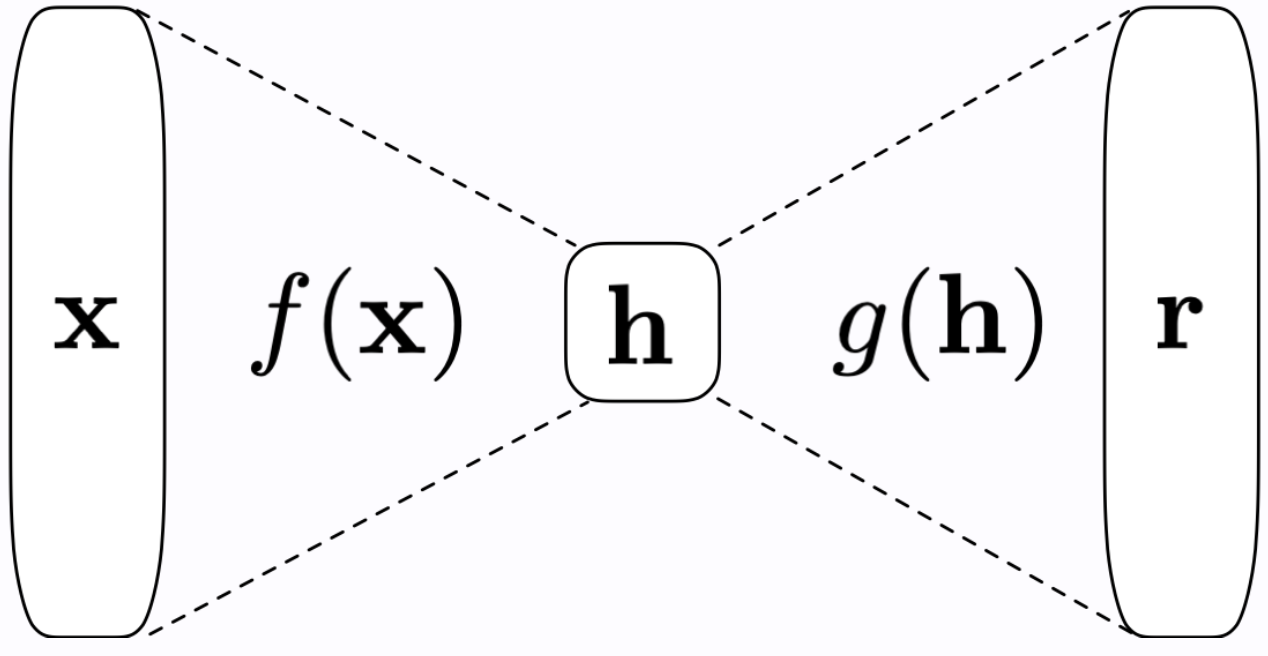
\includegraphics[scale=.4]{images/autoencoders/undercomplete.png}
\end{figure}


L'idea di questo primo tipo di autoencoder, l'undercomplete autoencoder è di utilizzare un solo modo di 
regolarizzare il riultato, cioè avere una hidden rappresentazione più piccola rispetto ai dati orginiali. 
La ricostrurizione di $x$ è chiamata a volte $\hat{x}$, a volte $r$.
\newline
\newline
Normalmente, l'idea alla base del learning process di un undercomplete autoencoder è la minimizzazione di una
loss function:
\begin{equation}
  L(x,g(f(x))),
\end{equation}
dove $L$ è una loss function che penalizza $g(f(x))$ se è troppo diversa da $x$ (ad esempio, la MSE).
In altre parole, usiamo una loss che prova a minimizzare la distanza tra l'input $x$ e l'output $g(f(x))$, 
cioè l'esempio ricostruito dall'autoencoder. 

\newpage
\subsection{Autoencoders e PCA} 
Esiste una connessione interessante tra undercomplete autoencoders e la PCA (tecnica di dimensionality 
reduction). Quando il decoder è lineare e $L$ è la MSE, un undercomplete autoencoder impara ad estendersi 
nello stesso sottospazio della PCA. Per capire meglio questo concetto, torniamo ricordiamo cosa è la PCA.

\paragraph{Sommario della PCA.}
La \textbf{Principal Component Analysis} può essere derivata da un algoritmo che \textbf{proietta ogni esempio
} $x$ in uno \textbf{spazio vettoriale di dimensione inferiore} con errore di ricostruzione minimo, cioè,
per la PCA:
\begin{equation}
  f(x)=\arg \min_h{||x-g(h)||_2},
\end{equation}
dove $g$ è una funzione di ricostruzione soggetta a \textbf{qualche costante}.
\begin{figure}[!h]
  \centering
  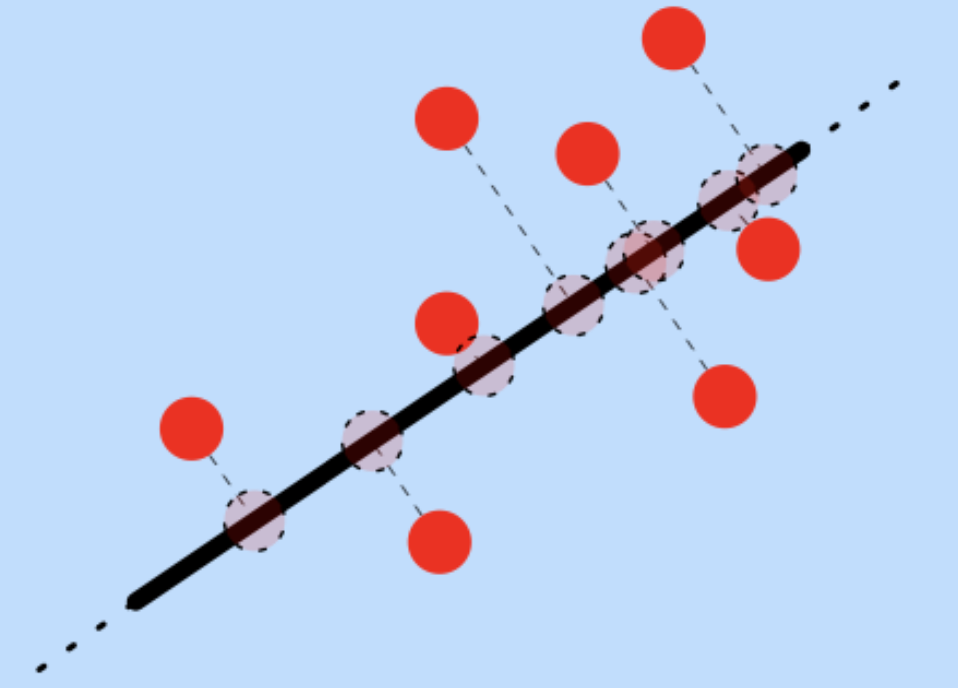
\includegraphics[scale=.4]{images/autoencoders/pca.png}
\end{figure}


In altre parole, l'idea è prendere i punti del dimensional space e proiettarli in uno spazio di dimenisonalità 
ridotta rispetto al primo. L'obiettivo della PCA è costruire una funzione $f$ che prenda in input $x$ e 
restituisca la sua rappresentazione nel nuovo spazio. $f(x)$ esplora tutte le possibili rappresentazioni di 
$h$ e sceglie quella che si avvicina di più ad $x$. Nel processo, viene anche fissata qualche costante.
\newline
\newline
Nello specifico, $g$ deve essere tale che :
\begin{itemize}
  \item $g$ sia \textbf{lineare}, vogliamo avere ad esempio $g(h)=Dh$, per qualche $D$, cioè che $g(h)$ 
  sia il prodotto matriciale $Dh$;
  \item le colonne di $D$ siano \textbf{ortogonali l'una con l'altra} (per semplificare il problema);
  \item le colonne di $D$ abbiano \textbf{norma unitaria} (per avere soluzioni uniche).
\end{itemize}


Con queste costanti, possiamo dimostrare che:
\begin{itemize}
  \item $f(x)=\arg \min_h{||x-g(h)||_2}=D^Tx=h_x$;
  \item $g(h)=Dh$,
\end{itemize}
che portano a:
\begin{itemize}
  \item $r(x)=g(f(x))=g(h_x)=DD^Tx$,
\end{itemize}
con $D$ \textbf{dato dagli autovalori} corrispondenti all'\textbf{autovettore più grande} della matrice 
$X^TX$.
\newpage

In sintesi:
\begin{itemize}
  \item un undercomplete autoencoder minimizza una loss tale che $L(x,g(f(x)))$;
  \item la PCA trova il mapping $f(x)=\arg \min_h{||x-g(h)||_2}$, imponendo che $g$ sia un modello lineare.
\end{itemize}


Dovrebbe essere evidente che quando $L=||\cdot||_2$ e il layer di ricostruzione è modellato da unità
lineari, abbiamo due approcci per risolvere lo stesso problema.


\subsection{Manyfold}
\textbf{Manyfold} è traducibile come \textbf{varietà}: consideriamo uno spazio con tante dimensioni,
diciamo tridimenisonale; se consideriamo solo due dimensioni, quei punti sono ancora nello spazio 
tridimenisonale ma sono anche in un sottospazio che ha una dimensione di meno. Pensiamo ad una sfera e ad 
un piano, in questo caso il piano è un manyfold bidimensionale immerso in uno spazio tridimensionale
(la sfera).
\newpage

\section{Regularized Autoencoders}
Anche in questo caso, viene utilizzata la size di $h$ come regularization factor. Ora però, la differenza tra
$h$ e l'input $x$ determina quanto l'autoencoder è forzato ad imparare solo le \textbf{parti più rilevanti 
dell'input}.
\newline
\textbf{Se $h$ è troppo grande}, l'autoencoder imparearà semplicemente la funzione identità.
\newline
E se invece $h$ ha dimensione $1$? Siamo sicuri di non stare costruendo semplice la funzione identità?
\newline
\newline
Infatti se l'autoencoder ha troppa capacità (o perché l'encoder e il decoder sono troppo potenti,
o perché il codice è troppo grande), non sarà in grado di apprendere nulla di utile.
\newline
Esamineremo ora gli \textbf{regularized autoencoders}: invece di limitare la capacità del modello mantenendo 
l'encoder e il decoder poco profondi e la dimensione degli hidden layer piccola, \textbf{si utilizza una 
loss function che incoraggia il modello ad avere altre proprietà} oltre a quella di copiare l'input nell'output.

\paragraph{Proprietà fruttate per la regolarizzazione.}
\begin{itemize}
  \item sparsità della rappresentazione $\Rightarrow$ \textbf{sparse autoencoders};
  \item robustezza al rumore o mancanza di input $\Rightarrow$ \textbf{denoising autoencoders};
  \item derivata piccola $\Rightarrow$ \textbf{contractive autoencoders}.
\end{itemize}

\subsection{Sparse Autoencoders}
\paragraph{Definizione.} Uno \textbf{sparse autoencoder} è semplicemente un autoencoder i cui criteri di 
allenamento includono una \textbf{penalità di scarsità} $\Omega(h)$ su layer di coding $h$, in aggiunta al
reconstruction error:
\begin{equation}
  L(x,g(f(x)))+\Omega(h).
\end{equation}
\begin{figure}[!h]
  \centering
  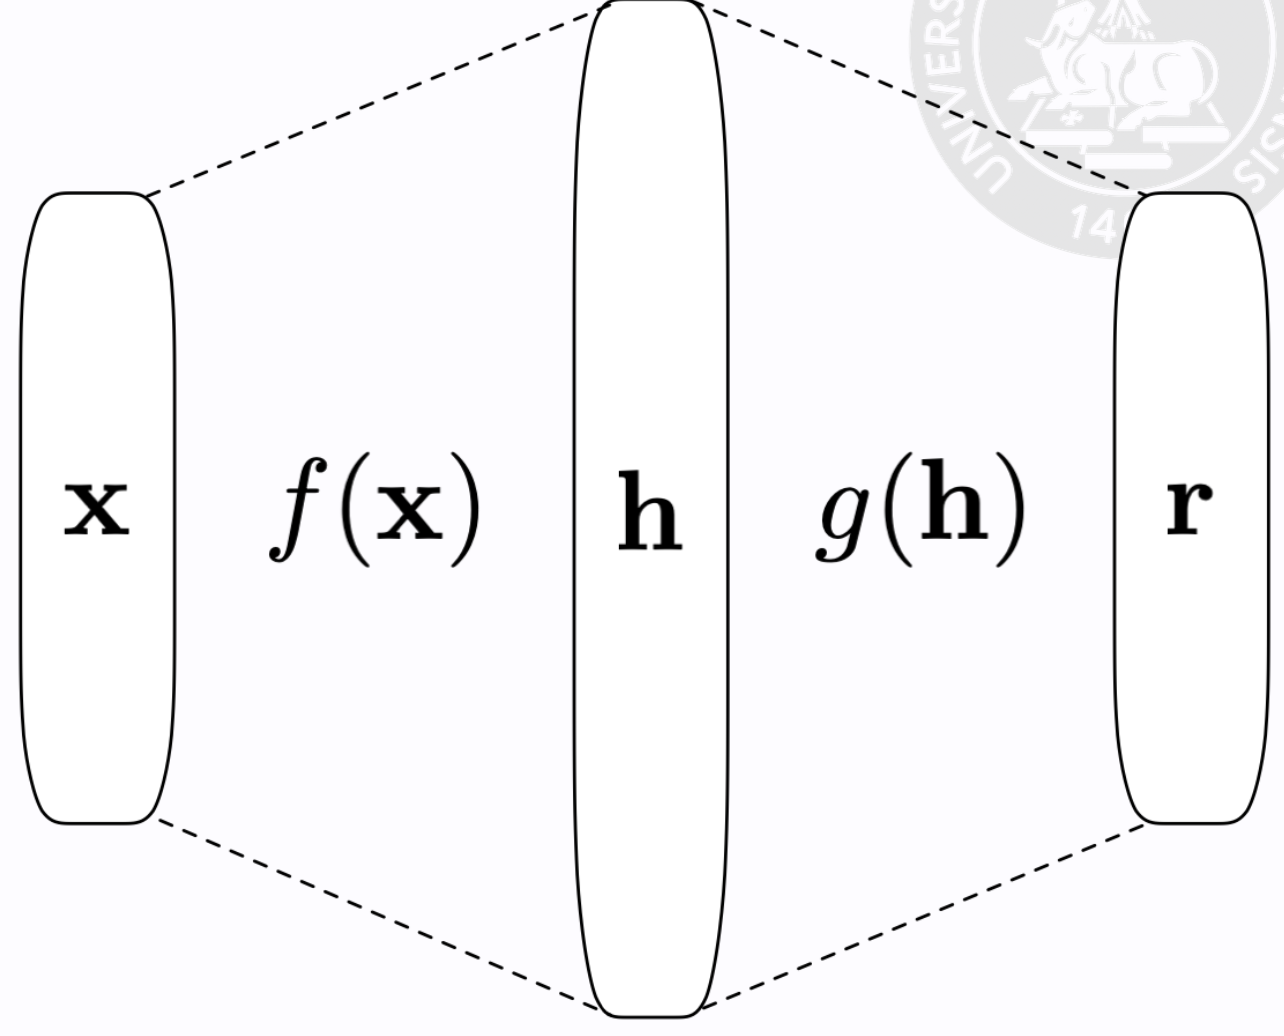
\includegraphics[scale=.4]{images/autoencoders/sparse_auto.png}
\end{figure}
\newpage

\subsection{Generative Models (GM)}
Esiste una connesione tra sparse autoencoders e generative models.
Un \textbf{generative model} è un modello che cerca di apprendere la distribuzione congiunta $p(x, y)$ dei 
dati. Dopo che il modello è stato addestrato, può generare nuovi punti di una determinata classe, 
campionando da essa. A volte $y$ non è una variabile osservabile. In questi casi, $y$ è chiamata 
\textbf{variabile latente} e solitamente è indicata con $h$.


I geneative models differiscono dai \textbf{modelli discriminativi}, poiché essi imparano ad approssimare 
la probabilità condizionata $p(y|x)$ e non possono quindi generare nuovi punti dati.
\newline
\newline
Supponiamo di avere un modello generativo con $x$ variabili visibili e $h$ variabili latenti, con una 
distribuzione:
\begin{equation}
  p_{model}(h,x)=p_{model}(h)p_{model}(x|h),
\end{equation}
dove $p_{model}(h)$ è la \textbf{distribuzione a priori del modello sulle variabili latenti}.
\newline
\newline
Sotto questi presupposti, la \textbf{likelihood di $x$ dato il modello} può essere calcolata come la 
marginalizzazione delle variabili latenti $h$:
\begin{equation}
  p_{model}(x)=\sum_hp_{model}(h,x).
\end{equation} 
\newline
\textbf{Importante:} $p_{model}(h)$ è un \textbf{prior differente} rispetto a quello normalmente assunto 
nei modelli probabilistici. Di solito il termine \textbf{prior} indica la preferenza di un algoritmo di 
apprendimento per una data soluzione (cioè per un dato modello) (\textbf{prior}) prima di vedere i dati.
Qui stiamo usando questo termine per \textbf{riferirci alla preferenza del modello per la rappresentazione 
latente $h$ prima di vedere $x$}.
\newline
\newline
Prendendo il logaritmo di $p_{model}(h)$ otteniamo la \textbf{log-likelihood} di $x$ nel modello:
\begin{equation}
  \log{p_{model}(x)}=\log\sum_hp_{model}(h,x). 
\end{equation}
\newline
\newline
Possiamo pensare all'autoencoder come un'\textbf{approssimazione di tale somma con una stima puntuale per 
un solo valore altamente probabile di $h$}.
\newline
\newline
Poi data una $\tilde{h}$ generata dall'encoder:
\begin{equation}
  \log{p_{model}(x)}=\log\sum_hp_{model}(h,x)\approx\log{p(\tilde{h},x)}=\log{p_{model}(\tilde{h})}+\log{p_{model
  }(x|\tilde{h})}.
\end{equation}
\newline
\newline
Ricordando ora che \textbf{gli sparse autoencoder sono allenati a minimzzare la loss}:
\begin{equation}
  L(x,g(f(x)))+\Omega(h),
\end{equation}
(dove il primo termine è la reconstruction loss e il secondo è la sparsity loss), possiamo vedere che, 
minimizzando la \textbf{reconstruction loss}, l'autoencoder sta imparando ad \textbf{approssimare la 
log-likelihood dei dati nel modello}.



Infatti, minimizzando la reconstruction loss, l'autoencoder sta imparando ad approssimare la probabilità
condizionata $p_{model}(x|h)$ poiché sta cercando di trovare $x$ che è la migliore ricostruzione dato $h$, 
cioè sta effettivamente risolvendo:
\begin{equation}
  \arg \max_p p_{model}(x|h)=\arg \min_x-\log p_{model}(x|h).
\end{equation}
\newpage

Se $\Omega(h)=\lambda\sum_i|h_i|$ (cioè usando la norma $L_1$ di $h$, \textbf{la quale incoraggia la 
sparsità}), la minimizzazione del termine di sparsità corrisponde alla massimizzazione della log-likelihood 
del termine $p(h)$ assumendo una Laplace prior su ogni componente di $h$, indipendentemente. Formalmente, se:
\begin{equation}
  p_{model}(h_i)=\frac{\lambda}{2}e^{-\lambda|h_i|},
\end{equation}
allora
\begin{equation}
  -\log{p_{model}(h)}=\sum_i\Big(\lambda|h_i|-\log{\frac{\lambda}{2}} \Big) = \Omega(h)+\text{const},
\end{equation}
dove $\lambda$ può essere trattata come un iper parametro e il termine costante, dipendente solo da $\lambda$,
non viene ottimizzato durante l'apprendimento e può essere ignorato.
\newline
\newline
Mettendo tutto insieme, allenare la rete a minimizzare il reconstruction error e la sparsity penalty equivale
ad allenare la rete a minimizzare la log-likelihood negativa dei dati del modello:
\begin{equation}
  \min{L(x,g(f(x)))}+\Omega(h)\approx\min{-\log{p_{model}(x)}}.
\end{equation}
Da questo punto di vista, la sparsity penaly non è un fattore regolarizzante: è solo la conseguenza 
della modellazione della joint distribution tenendo conto delle variabili latenti e assumendo che esse 
abbiano la Laplace prior.
\newline
Questo punto di vista fornisce diverse motivazioni per il training di sparse autoencoder:
\begin{itemize}
  \item è un modo per addestrare approssimativamente un modello generativo;
  \item le feature imparate sono utili perchè descrivono le variabili latenti che spiegano l'input.
\end{itemize}
\paragraph{Designing output units}
Progettare le output units ci fornisce una connesione per giustificare la definizione dei
prossimi tipi di autoencoders. Nel seguito giustificheremo la scelta di utilizzare particolari output units.
\newline
\newline
Una strategia generale per progettare le \textbf{output units e la loss function} di una rete feedforward è di
interpretare la rete come il calcolo di una distribuzione $p(y|x)$ e la minimizzazione della log-likelihood
negativa $-\log{p(y|x)}$.


\textbf{Nel caso degli autoencoders}, $x$ è anche il target, oltre ad essere l'input. In ogni caso, possiamo
sfruttare la stessa idea.
\newline
Potremmo vedere il decoder come il fornitore della distribuzione condizionata $p_{decoder}(x|h)$.
\newline
\newline
Nel caso in cui $x$ sia un valore reale, \textbf{adottare linear output units e una loss quadratica} 
corrisponderebbe a massimizzare $p_{decoder}(x|h)$ sotto l'assunzione che la probabilità si distribuisce come 
$\mathcal{N}(x;\hat{x},mathbf{I})$, con $\hat{x}$ fornita dal linear layer output: $\hat{x}=Wh$. Cominciamo
ricordando che la probabilità di una distribuzione normale multivariata, di parametri $\mu$ e $\Sigma$, 
è data da:
\begin{equation}
  p(x)=\frac{1}{(2\pi)^{n/2}|\Sigma|^{1/2}}\exp{\Big(-\frac{1}{2}(x-\mu)^T\Sigma^{-1}(x-\mu) \Big)},
\end{equation}
che porta a
\begin{equation}
  p_{decoder}(x|h)=c_1\exp{\Big(-(x-Wh)^T\mathbf{I}(x-Wh)\Big)}=c_1\exp{-||x-Wh||^2},
\end{equation}
implicando che minimizzare la loss quadratica equivale a massimizzare la log-likelihood dei dati del modello,
siccome:
\begin{equation}
  -\log{p_{decoder}(x|h)}=||x-Wh||^2+c.
\end{equation}
\textbf{Nota:} visto che le linear units non saturano, non creano nessun problema agli algoritmi di ottimizzazione
basati su gradienti.
\newpage

\textbf{slide 30}:x è un vettore di valori reali,  se adortiamo linera units e quadratic loss è uguale ad assumere che la prob 
distr di x|h è una normal distr. dove mean is e variance is id matrix

\textbf{slide 31}: qui parliamo di x contenenti valori booleani 0 1, possiamo mostrare che possiamo 
assumere che 

\textbf{slide 32}: possiamo guardare l'Autoencoders come, l'encoder come modelling a distrubition di h|x
e l'encoderr come x|h. questo esempio mostra che fare questo tipo di modelling da qualche suggeriemtno.
l'encoder pul essere pensato come abbiamo detto e il decoder uguale, il punto è che non c'è motivo

\textbf{slide 33}: una ragione per parlare di questo tipo è che si pul dimostrare che l'encoding e il decoder
corisèondon alle prob di prima ma son coerenti tradi loro e sono due facce dello stesso modello, cosa che
prima non era garantita ma ora lo è. p un risltato teorica che non dimostriqmo.

\textbf{slide 35}: l'idea èc he l'unica cosa che cambia da prima 

\textbf{slide 36}:

\textbf{slide 37}:

\textbf{slide 38}:

\textbf{slide 39}:

\textbf{slide 40}: 

\textbf{slide 41}:

\textbf{slide 42}: possono essere compleyamente descritte da.. se pensiamo ad un punto nel manifolds 
è un pumnto tangente al piano. il punto è che una priprietà intressante tehi tangenti palc3s 
they ti danno la direzione nell'higheri dimenisonal space in cui si può viaggiare di più senza 
lasciare il manyfolders 

\textbf{slide 43}: 

\textbf{slide 44}:

\textbf{slide 45}: 

\textbf{slide 46}: 

\textbf{slide 47}: l'idea dietro i denoising Autoencoders è intuitiva, qua no. a contractive Autoencoders 
è un regularised Autoencodersche rpvoa a minimizzare una loss functian di questo forma (guarda forma nella 
slide) la forma partiolcare di questa regularisxation term è deove c'è lambda. quello che dice è che pupi 
pensare ad x come una funzione da x a h dove h è un vettore di copmonenti h1,h2,hk e f èuò esser evista 
come yna funzione ch eha muyltid imput e multid output. f è composta quindi dall'unione di k difeferenti 
funtion una che costrusce h1, una h2. abbiamo il gradient rispetto ad x di ogni termine h. il regolarization
term ci dice che uole tenere tutte le derivate parziali piccole. 

\textbf{slide 48}: se abbiamo un lamba molto molto alto, qual è la soluzione? quale tipo di funzione 
andremo ad imparare? è un piano (?) costante

\textbf{slide 49}: qua diciamo che possiamo riscrivere lo stesos oggetto omega in un altro modo

\textbf{slide 50}: se guardimo la variazione nello spazio originale e  in quello embedded il modello cercherà
di mappare le variaizoni dello spazio originale in piccole variazioni in quello embedded.
per capire perchè guardiamo le due funzioni nella slide. il denominaroe serve per avere funzioni da 
plottare semplicemente. se prendiamo un range di bvalori nel space, quando la derivata è piccola, 
come nella qudratuca fun, oer lo stesso range se guardiamo l'output, nel caso della quadraica il range di 
valori è molto pià piccolo di quello della cubica.

\textbf{slide 51}: menzioniamo solo il fatto che queste prorpietta contratticve valgono solo localmente.
quindi se si fanno un certo unmero di passaggi possiamo avere due punti distanti di pià nell'emebdding space
che nello spazio oringiale.

\textbf{slide 52}: c'è un paper che mostra che se assimuamo uno small gaussian imput noise, allora la 
recostruction è equivalente ad una crontative penaltu on the recontractuve function. la differenza è che
vedere la slide.

\textbf{slide 53}: già detto

\textbf{slide 54}: da qualsisai direzione dello spazio calcoliamo il prpodto tra il jacoviano e la direzione
abbiamo un prodotto grande quando la direzione è allineata alla direzione in cui la h cambia di più. 
queste direzioni sono quelle che vengono penalizzate dalla penalità contrattiva. quindi le direzioni che 
sopravvicono sono quelle lungo il manifolds. rimanogno quelle in cui cresce di più perchè sono quelle
che più descrvono i dati.

\textbf{slide 55}: un variational Autoencoders regolarizano la encoding distribution e ciò singicia 
rendere un Autoencoders buono come generative model. se proviamo a ottimizzare così, è troppo diffiicle
da fare quindi assumiamo che la distruvizione abbia nuna partioclare forma facile da ottimizzare. a quel punto
cerchiamo di approssimare quanto meglio possibile.

\textbf{slide 56}: partiamo da peerchè abbiamo bisogno di var Autoencoders, focus sui simple Autoencoders,
e proviamo ad usarlo come generative model. durante il training facciamo tutto come al solito, x, costruisamo
h e ricostruiamo x nel last layer del decoder. per usare questa astchietettura buttiamo via l'encoding part
e cominciamo a genereare ogni vettore randomicamente. poi cerchiamo di ricostruire l'input da questi random
vector. 

\textbf{slide 57}: questo succede. a sinisttra abiamo le ricostruizioni dei mnist digit fatti da un 
Autoencoders quando le vengono verniti gli h. a destra abbiamo il risultato dell'estrazione dei h vettori
random. perchè succede?

\textbf{slide 58}: il punto è che non c'è niente nel Autoencoders definition data fino ad ora che forzi
l'embedding space ad essere copmatto e ad avere un significato. l'idea è di regolarizzare la distribuxione
dei punto nell'emebdding space così da compattarli. 

\textbf{slide 59}: l'idea principale è che abbiamo gli usual Autoencoders, quindi metà Autoencoders function,
g che finzionpa come decoder funciton. la noviutà è che f non vuilda direttamente h, builda un vettore 
di 2 pezzi che specidica la media e la varianza di una distrivyzione normale. il punto è che startiamo con
l'immagine, abbiamo una mu e una sigma associata ad ogni image e l'idea è che nell'e,bedding space tutti i 
punti vicini a questa media e varianza corrispondano a qualche tipoi di.. quindi sampling da una normal 
distribution.

\textbf{slide 60}: 

\textbf{slide 61}: rimane un problema intrattabile anche con queste assunzioni. 

\textbf{slide 62}: 

\textbf{slide 63}: dobbismo ancora fare qualche operazione. non sappiamo ancora come ottimizzare g, la decoder
function. per ottimizzare g ptoviamo ad ottimiazzare p(x|h), qunidi trovare argmax di expection rispetto alle
h distrivutie comele qx(h) del log di p(x|h). il log di p() è il termine usato prima, possiamo quindi mettere
tutto insieme nel problema di ottimizzazione. kl non dipende da g, ma il primo termine si. cambiamo il meno
in più così abbiamo un problema di minimizzazione. è una regularize network con ilr ecustruct term e il 
regolaritzation term.

\textbf{slide 64}: abbiamo ancora il problema che nella nosta idea originale dobbiamo fare sapmling per
generare h. il problema è come differenziarli. la soluzione è la reparamtroization trick. a gausiiana con
parametri mu x e sigma x +è esattamente la stessa di una random normal ida cui faccaimo sampling e poi 
riscaliamo. non estraiamo dalla prima normale, che dipendeno da sigma x e mu x che dipendono dalla nosyta rete,
ma dalla seconda normal 0 e 1, riscalo e ottengo una serie di dipendenze che permette di derivare h e mu e x
continuando la backpropagation. non riesco a calcoalre le derivate della parte che contiene il sampling ma
nomn ci interessa quella parte della rete. 

\textbf{slide 65}:

\textbf{slide 66}:

\textbf{slide 67}:

\textbf{slide 68}: 

\textbf{slide 69}:

\textbf{slide 70}: